\chapter{Project Results }

\section{Physical objective}
The objective of this project is to construct an autonomous robot based on the line follower project from the labs of the Digital Systems B course. The robot has to not only utilize IR sensors to follow the line but also be able to pass the challenges outlined below while navigating through the map (sometimes referred to as "the maze"), as described in Chapter 1 of the project manual.\\
The routing algorithm is executed on the computer that communicates with the robot through UART and XBee wireless modules, which completes the entire autonomous system.\\

\begin{itemize}
    \item In the first challenge the robot has to visit a series of stations in the given order.
    \item The second challenge consists of the first one and the addition of "mines" which are metal disks that have to be avoided by the robot.
    \item During the last challenge more mines will be placed in the maze and the robot has to find them all. In stage 2 a new mine will be added and the robot has to find it also. 
\end{itemize}
%fuck it
The structure of the robot is shown in figure 1.2 of the project manual and summarized here in the figure below.

\begin{figure}[h!]
    \centering
    \resizebox{\textwidth}{!}{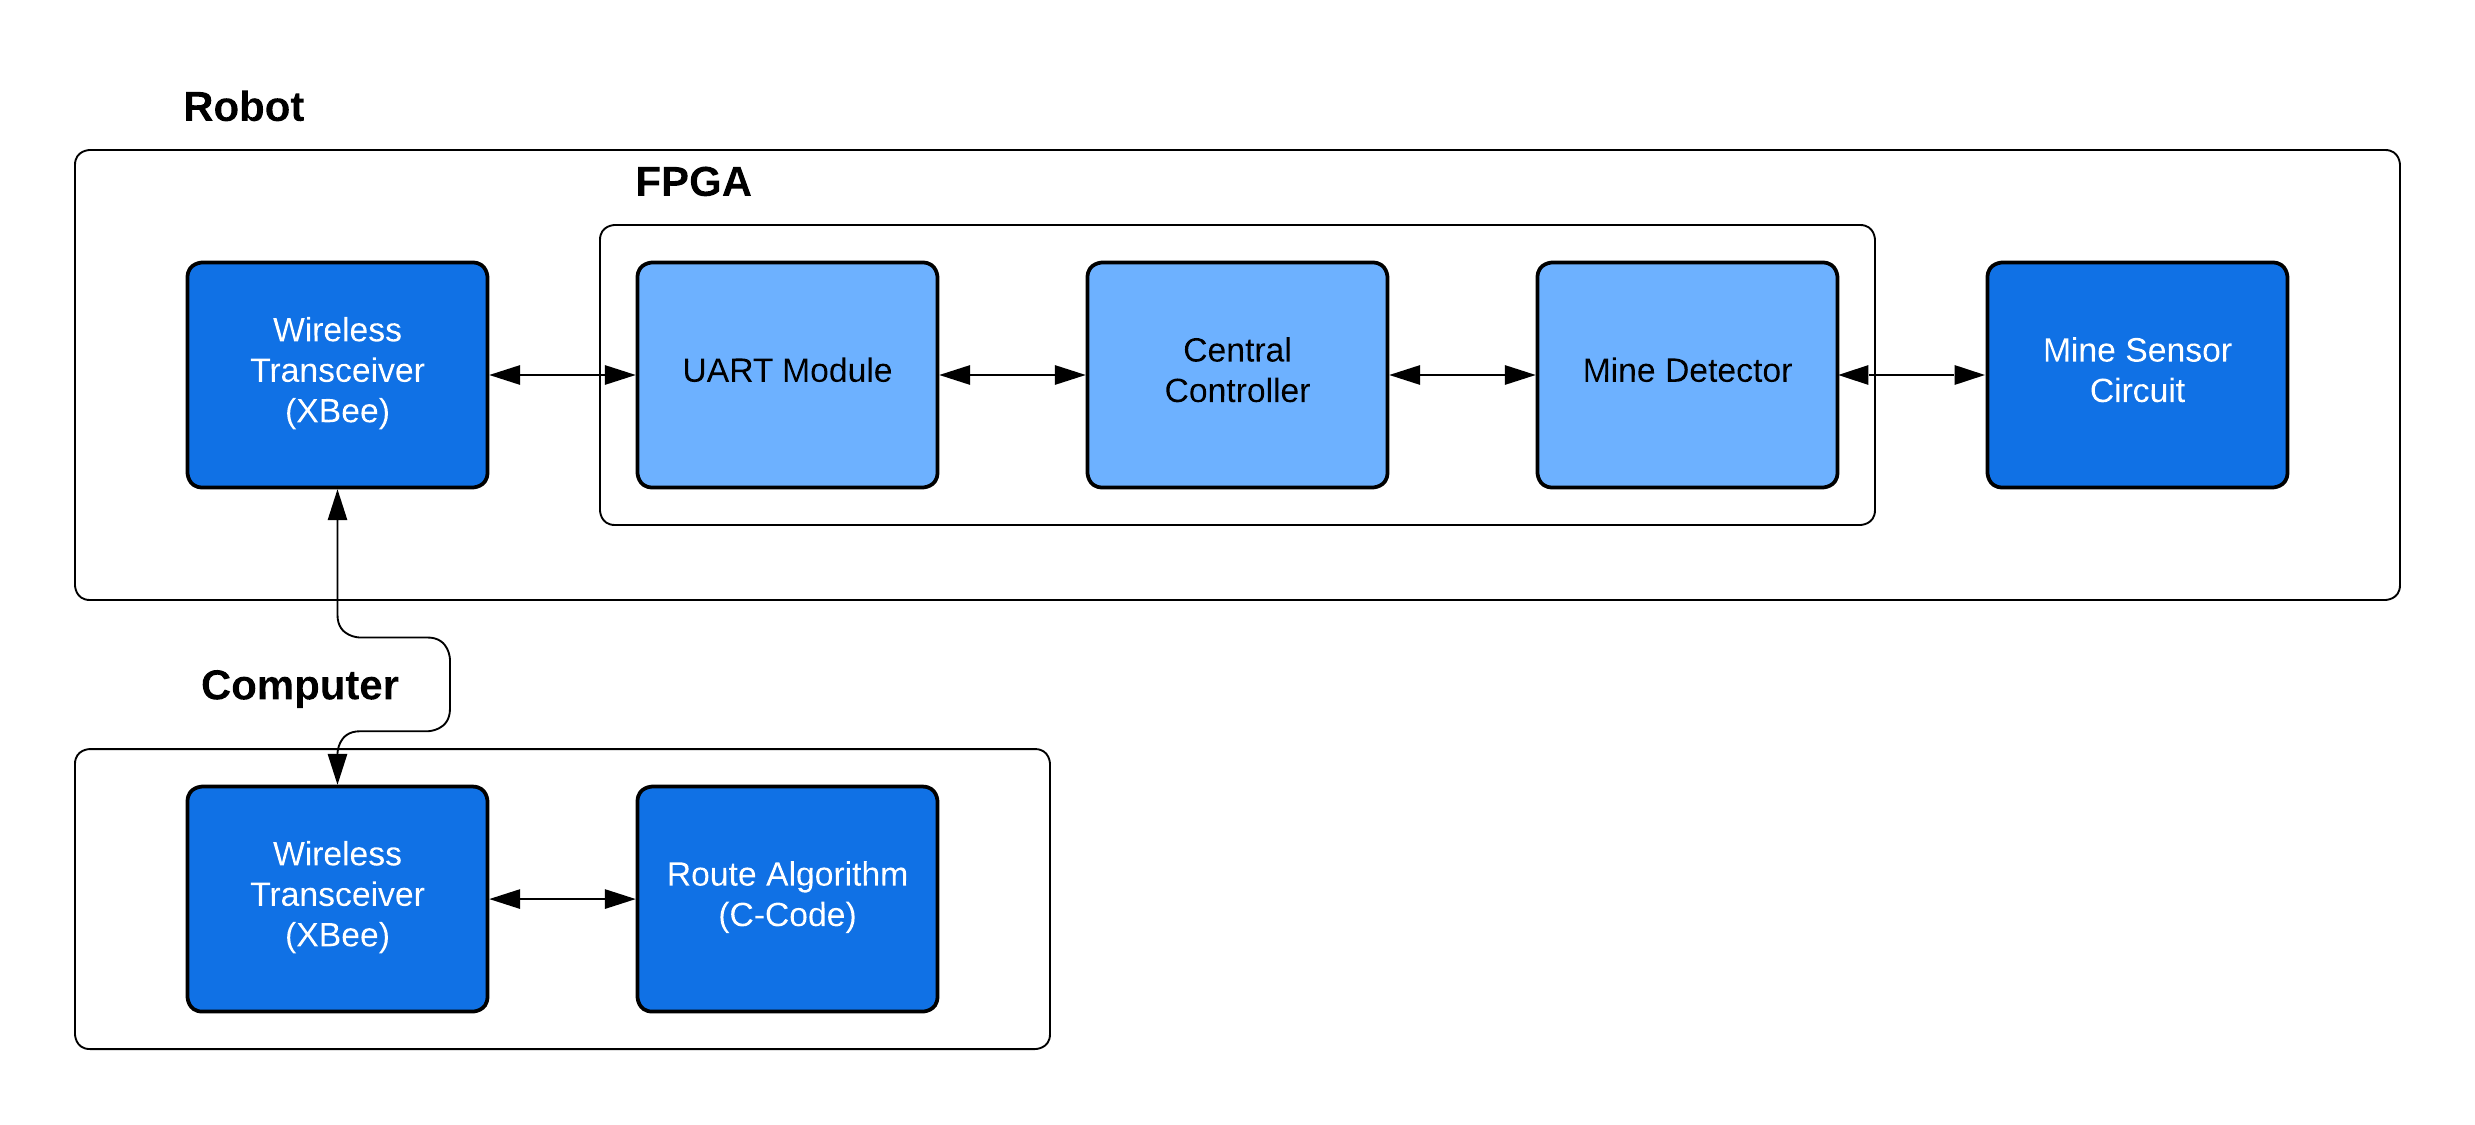
\includegraphics{Flowchart (2).png}}
    \caption{Block diagram of the entire system.}
    \label{fig:block}
\end{figure}

\newpage
The workload was split into the following parts that correspond to every subgroup in the project:\\ 
\iffalse
The aim is to construct a loudspeaker system with a flat response due to the accuracy and quality of the filters, the amplifier, and the power supply.\\
We should be able to plug the speaker in and have music come out of it. The music should be split between 3 speakers: high frequencies come out of the tweeter, middle frequencies come out of the mid-speaker, and low frequencies from the woofer.\\
We should also be able to have an additional active filter for the bass level.
\fi

\begin{itemize}
    \item VHDL: The FSM is already written in VHDL to perform the line-follower assignment in which the test robot follows the black line. The line follower’s FSM needs to be extended or completed in order to complete the functionality of the robot. The robot needs to detect a mine for example. After the FSM has been made it needs to be written in VHDL.

    \item C code and Serial Communication: The main objective of the serial communication part is to create an interface that can guide the robot via the PC. This will be done using the XBee modules that communicate with each other with the ZigBee protocol and with the external hardware via a UART protocol. To achieve this we will write a small application in C (programming language)  for the laptop and a corresponding VHDL program for the robot.
    
    % C-group task description:
    \item C-code: The objective for the smart robot is to create a separate program with a simple user interface. This program will be implemented into a larger program that will control the robot. We will describe a algorithm that can be used to compute the route through the maze and also a data structure to implement this algorithm. 

    \item Mine detector: One of the important aspects of the smart robot is the ability to detect mines in their path when going from position A to position B. The robot must detect the mines and avoid them and thus redetermine a new path. In order to detect them a mine detector sensor must be built. This sensor must also be able to roughly determine the mine distance to the robot. It will be implemented using an LC oscillator.
\end{itemize}


\section{Learning objectives}
Besides creating a working autonomous robot system, the goal is to master certain learning objectives of the EPO project.\\ 
After completion of the project, we will be able to apply the theoretical concepts of the first year in practice. Another important aspect is that we will be able to methodologically design an electronic system utilizing a project-based team approach.
\iffalse
Next, we have to achieve the basics of working in an engineering project group. the basics consist of planning, creating well-organized meetings, writing project plans, having the ability to give presentations, and writing engineering reports.\\
\fi
At last, we will learn and practice critical thinking and the ability to find information in relevant sources such as datasheets and manuals, as well as critically assess and utilize those pieces of information.


%\figure[scale=0.17]{Flowchart (2).png}